\label{chapter:lowlevel}
\textit{Chapter 2 exposes the design of the low-level architecture of the mobile robot. The low-level architecture is supported by an Teensy micro-controller. This platform is connected to the main sensors and components of the robot and processes the raw data coming from: IMU, GoT, motor encoders, battery, motors and ultimately the RaspberryPi. The following sections present the main program of the Arduino Teensy handling raw data from sensors and transforming it into useful information about robot's position, orientation and motion.}\\

One of the most important characteristic of an autonomous robot is to know its position in the Cartesian space. Such information is characterized by 3 translational quantities ($x$, $y$, $z$) and 3 angular quantities ($\theta_x$, $\theta_y$, $\theta_z$).\\

A differential drive 2D mobile platform can translate on 2 dimensions $x$, $y$ and rotate on one dimension $\theta_x$. The robot has 3 degrees of freedom (DOF) and its pose is characterized by ($x$, $y$, $\theta_x$). These quantities have to be calculated from the sensors used on the robot.\\

Lastly, localization based on sensors is a kinematic approach to modelling the robot's translational and angular motion. This means that its pose is described by a function of wheels' movement and robot's motion disregarding the forces and moments that make it move (dynamics approach).\cite{robotics}\\ 

\section{Local and Global Robot Positioning}

\textit{This section explains the algorithms to determine the translational position of a 2D mobile robot using 2 sensors: encoders and ultrasonic global positioning system (GoT).}\\

Translational quantities are determined by the use of encoders for local positioning and GoT for global positioning. It follows that 2 noisy sensors providing redundant information can be fused together to output a better estimate of the translational position of the robot. Sensor fusion can be computationally heavy and is considered in this project a high-level task and will be described in Chapter \ref{chapter:highlevel}.\\


\subsection{Odometry and Dead-Reckoning}

Odometry or localization-by-odometry is used to calculate the robot's position using the encoders mounted on each wheel. The robot has a differentially-steered drive system, meaning that each of the 2 wheels can be independently powered and controlled providing different steering functions. \cite{robotics}
The logic behind differential-steering drive systems is simple:


\begin{enumerate}
    \item wheels move in tandem \textbf{--->} robot moves forward;
    \item right wheel moves faster than left \textbf{--->} robot yaws to left;
    \item right wheel moves slower than left \textbf{--->} robot yaws to right;
    \item wheels move in opposite directions \textbf{--->} robots spins around its axis.
\end{enumerate}
\\

The understanding behind localization by odometry is also simple, for example, a robot starting at an origin point (0, 0) and moving with 1 meter per second (m/s) for 3 s only on the x-axis should be at (3, 0) as a final position. \cite{mit} These simple position estimates are based on wheel revolutions and their speed of turning - how many revolutions per second. Wheel revolutions are calculated based on encoder readings (or ticks) - how many ticks per revolution. These ticks depends on the type of encoder and its technical specifications.\\

The type of encoders used in this project are quadrature phase encoders that have 2 simple encoders producing 90 degrees out-of-phase wave-forms. These type of encoders are used because the direction of spin can be calculated easily depending on the leading signal: if one signal leads then the motor rotates clockwise, if the other one leads then it rotates counter-clockwise. Knowing the spin direction allows knowing if the robot moves forwards or backwards. In the code Listing \ref{code:encoderticks} can be seen how the spin direction can be calculated. This type of encoder with 2 signal waveforms is shown in Figure \ref{figure:encoder}.

\begin{figure}[H]
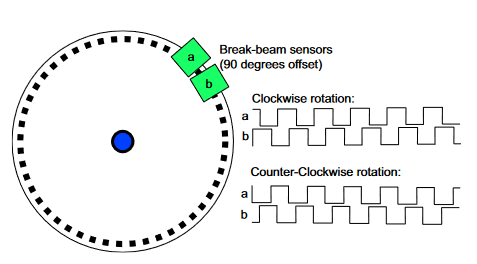
\includegraphics[scale=0.75]{Figures/encoder.PNG}
\centering
\caption{Illustration of a quadrature phase encoder and the 90 degree out-of-phase waveform necessary to detect motor direction. Source: \cite{mit}}
\label{figure:encoder}
\end{figure}

Encoders have to be read using the interrupt capability of the micro-controller in order to allow other programs to run while reading the encoder. The interrupt function can be called for one or both signals of the encoders - the encoder's specification giving the number of cycles per revolution, as seen in Chapter \ref{chapter:intro}, 64 CPR refers to both channels. If only one channel is connected to the interupt pin, the cycles per revolution is halved. In this project, as can be seen in Listing \ref{code:encoderticks}, only one channel is connected to an interrupt pin.\\
  
\begin{lstlisting}[language=C++, caption={Encoder ticks count for determining motor spin direction. If the count is increasing, then the motor is driving forward and vice-versa.}, label={code:encoderticks}]

// defines interrupt pin for signal A of right-hand encoder
#define RH_ENCODER_A 2
// defines interrupt pin for signal B of right-hand encoder
#define RH_ENCODER_B 3

// initialize hardware interrupts for one channel
attachInterrupt(2, readRightEncoder, CHANGE);

  if (digitalRead(RH_ENCODER_A) == HIGH) {
    if (digitalRead(RH_ENCODER_B) == LOW) {
        Count++;
    } else {
        Count--;
    }
  } else {
    if (digitalRead(RH_ENCODER_B) == LOW) {
        Count--;
    } else {
        Count++;
    }
  }

\end{lstlisting}
  
The speeds of motors can give information about two quantities: rate of moving forward and rate of turn of the robot - these two are the linear and angular speeds, which integrated give the linear and angular position of the robot ($x$, $y$, $\theta_x$). Since these two quantities do not have analytical expression to calculate the integral, the values are integrated numerically - divide time in very small intervals in the order of milliseconds and add all the quantities over the period of time. \cite{mit} \\

Before showing the kinematic equations, it is important to mention the assumption on which these equations work. It is further assumed that the robot has a constant velocity and there is no acceleration present. Acceleration effects are neglected. \cite{robotics}\\

Suppose the robot starts from position (0, 0, 0) at time $t_0$ then its pose changes with time $t = t_0 + \Delta t$ for every $\Delta t$ - where $\Delta t$ represents the time interval between position updates. If $d_{left}$ and $d_{right}$ represent the distance of the wheels traveled in $\Delta t$ the following the logic of differential-steer drive mentioned above, the robot moves:

\begin{enumerate}
    \item $d_{right}$ = $d_{left}$\textbf{ ---> }robot moves forward;
    \item $d_{right}$ > $d_{left}$\textbf{ ---> }robot yaws to left;
    \item $d_{right}$ < $d_{left}$\textbf{ ---> }robot yaws to right;
    \item $d_{right}$ > 0 and  $d_{left}$ < 0\textbf{ ---> }robot spins around its axis.
\end{enumerate}

Determining the robot's pose when moving forward is as simple as the example in the beginning of the section, however determining the pose when the robot is turning requires arc geometry. The assumption is that the robot's trajectory is an arc. Starting at an initial state ($x_0$, $y_0$, $\theta_0$), after moving $\Delta t$ period of time, the new pose ($x$, $y$, $\theta$) can be calculated.\\

The robot is a rigid body and if the robot changes position, all points on the robot change position and velocity. Following the midpoint on the distance between the two wheels (baseline) as the robot moves, the midpoint coordinates gives the robot's position. Hence, the length of the arc traveled by the robot at the midpoint is given by:

\begin{equation}
    d_{midpoint} = \frac{d_{left} + d_{right}}{2}
\end{equation}

where the arc length is also given by the the radius of the circle formed by each wheel, $r_{left}$ and $r_{right}$ multiplied with the angle formed $\phi$, giving the following equation for each wheel:

\begin{equation}
    \phi r_{left} = d_{left} 
\label{eq:radius_left}
\end{equation}

\begin{equation}
    \phi r_{right} = d_{right}
\label{eq:radius_right}
\end{equation}

Setting a frame of reference on the left wheel, then the $d_{midpoint}$ can also be written as the difference between $d_{right}$ and $d_{left}$. The equation of traveling in an arc for the midpoint becomes:

\begin{equation}
    \phi r_{midpoint} = d_{midpoint} =  d_{right} - d_{left}
\label{eq:radius_midpoint}
\end{equation}

By substituting Equations \ref{eq:radius_left} and \ref{eq:radius_right} into \ref{eq:radius_midpoint}, the radius quantity is canceled and the angle $\phi$ depends only in the distance travelled by the left, right wheel and midpoint. The odometry geometry can be seen in Figure \ref{figure:geometry} where all quantities explained before can be seen. The odometry equations used to calculate the (x, y, $\theta$) are shown below:


\begin{equation}
    x = x_0 + d_{midpoint}\cos{\theta}
\end{equation}

\begin{equation}
    y = y_0 + d_{midpoint}\sin{\theta}
\end{equation}

\begin{equation}
    \theta = \theta_0 + \phi
\label{eq:theta}
\end{equation}

\begin{figure}[H]
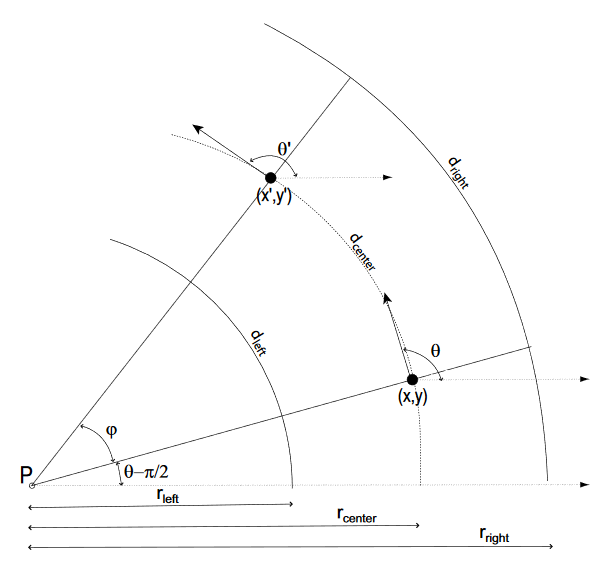
\includegraphics[scale=0.75]{Figures/geometry.PNG}
\centering
\caption{Odometry geometry. The arc length created by left wheel, midpoint and right wheel have the same center point $P$ but different radia: $r_{left}$, $r_{midpoint}$, $r_{right}$. Robot's heading is given by angle $\theta$ while angle $\phi$ is the inner circle angle formed by angular motion. Source: \cite{mit}}
\label{figure:geometry}
\end{figure}

As mentioned above, odometry describes the local position of the robot, relative to a starting point. This means that it cannot be used in a map for global positioning without knowing its starting position.\\

Moreover, odometry calculations grow inaccurate with time due to wheel slip, misread ticks, unlevel surface and asymetrical wheels. To compensate for this error, data from another sensor can be used. In this project, data from a global positioning system is fused with odometry to get the best positioning estimate of the robot.


\subsection{GoT Positioning}

\textcolor{red}{Briefly describe trilanteration, global positioning based on satellites}

\subsection{Sanity Check}

Sanity checks are tests used to evaluate a claim in a basic manner. The claim to check in this section is the inaccuracies of the odometry calculations versus the global positioning system.\\

On a flat surface marked by a ruler, the robot travelled  2 meters from a known position by the GoT system. The position was added as bias in the odometry starting position and the resulting (x, y) graph plotted real-time through serial communication in Matlab can be seen in Figure \ref{figure:sanitycheck_got}.

\begin{figure}[H]
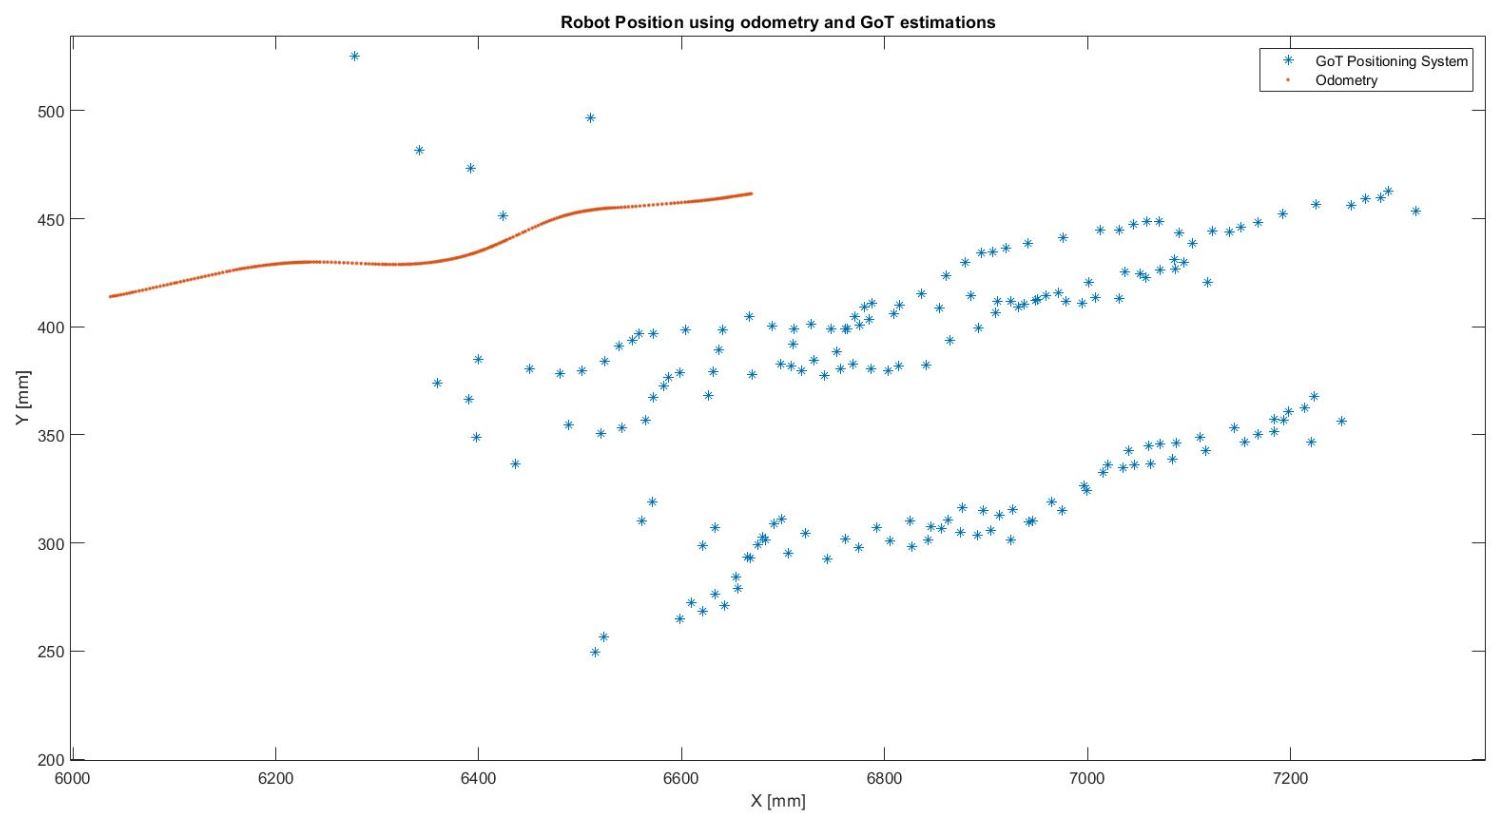
\includegraphics[scale=0.45]{Figures/sanity_check_got.jpg}
\centering
\caption{Robot position estimation through encoders versus GoT system. Inaccuracies of the GoT system (blue) are the most striking especially because of the double estimations seen in blue. These double estimations happen due to the fact that an obstacle was present near the robot at all time: the PC capturing the serial communication.}
\label{figure:sanitycheck_got}
\end{figure}

\textcolor{red}{Serial comm sucks. Chuncks of the graph are missing. Need to redo this graph -- use write to file NOT serial read.}\\

The results of the sanity test confirms that both sensors provide inaccurate measurements of the robot position and sensor fusion would be able to provide the best estimate between the two. The increasing value on the y-axis are an error which can be corrected by more aggressive PID controller than the current one - the small curvatures on the graph are the gains of the controller acting on correcting the position.


\section{Robot Orientation}

This section shows how to obtain the robot's orientation or angular position in a Cartesian space. In this project, the heading is obtained from 2 noisy sensors: the encoders and magnetometer. Sensor fusion between these 2 streams of data is considered in order to reduce the accumulation of error from encoder readings and interference errors from the magnetometer.\\

\subsection{Encoder Heading}

As mentioned in the section above, the heading of the robot is also calculated based on kinematic equations. Equation \ref{eq:theta} updates the heading of the robot based on its motion and it has to be bounded between [0, 2$\pi$] as in Listing \ref{code:theta}.

\begin{lstlisting}[language=C++, caption={Robot heading update equations}, label={code:theta}]
	
	double phi = (dRight - dLeft) / (double)dBaseline;
	theta += phi;
	if (theta > 2.0 * pi) theta -= 2.0 * pi;
	if (theta < 0.0) theta += 2.0 * pi;
	xPosition += dMidpoint * cos(theta);
	yPosition += dMidpoint * sin(theta);
	
\end{lstlisting}

The odometry equations assume that the robot performs the angular motion in two phases: first, rotate in place so that the heading matches the desired angle, then move in a straight line. \textcolor{red}{This assumption does not hold currently for the robot but as long as $\phi$ is small, these distances can be neglected. Using current code, the robot first has to align heading towards goal and then move in a straight line. However, now with the encoders we can rotate in place just like roomba. TO do this, we have to get heading from magnetometer, send opposite pwm to wheels to rotate in place up until heading is towards the goal. This may also be the out.of.the.box implementation of ROS. Continue writing on the next section when the ROS framework is in place. Low-level architecture should only deal with sending sensor data and writing pwm to motor. No position or heading calculation should happen low-level. Lowlevel fiddling should be kept to a minimum. Base design on this.} 

\subsection{Magnetometer-based Heading Relative to Target Position}

%we only know the heading of the robot relative to given target but don't know robot's heading %relative to true north
\textit{This section describes the algorithm implemented to calculate robot's orientation relative to a given target position. This is done by reading the magnetometer and calibrating it for accurate robot orientation, process target position and calculate the difference between actual and desired heading}.  
 \textcolor{red}{this section depends on the ros framework, we may not need it.}

\subsection{Magnetometer Calibration}
In the section before, the robot's position is calculated by the GoT system. This system does not provide information about the heading of the robot nor its speed. In this section, the algorithm for calibrating magnetometer's reading is described.\\

As robot orientation is crucial for path planning, a magnetometer is used to calculate the heading. The magnetometer is a sensor sensitive to Earth's magnetic field strength and outputs its heading relative to Earth's magnetic pole\footnote{Earth's magnetic field is similar to a dipole magnet. The field originates from a point close to the south pole and terminates at a point close to the north pole - see Figure \ref{figure:earthref} (a). These points are the magnetic poles. The geographic and magnetic poles are not the same - a difference of 11.5 degrees exists between the two. This angle can be added to the magnetic calculations knows as \textit{declination angle} so that the magnetometer shows the heading relative to true north}. The magnetic field lines vary in strength and direction about Earth's plane and is represented as $H_e$ in Figure \ref{figure:earthref} (b) by the three axes $H_x$, $H_y$, $H_z$. \cite{magnetometer} \\

\begin{figure}[H]
	\begin{minipage}{0.48\linewidth}
		\centering
		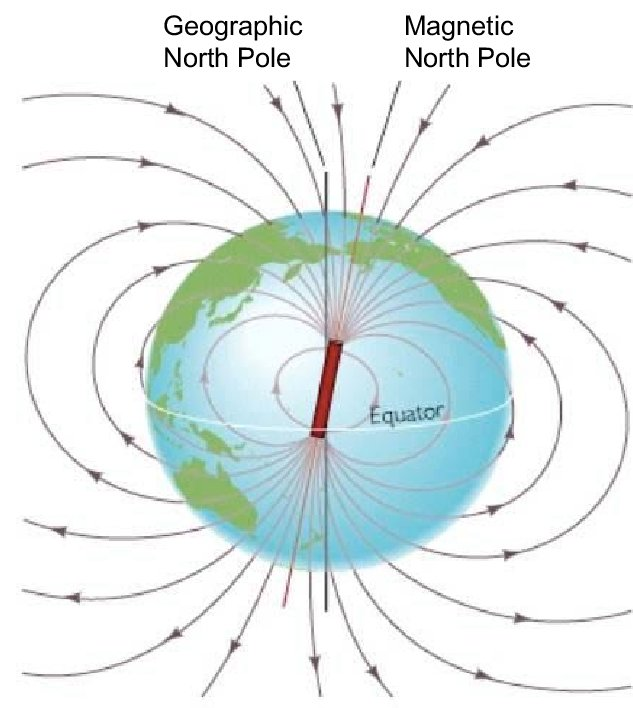
\includegraphics[width=\textwidth]{Figures/magneticfield.jpg}
		\caption*{(a) Earth's Magnetic Field. Source: \cite{filipski2006nanosatellite}}
	\end{minipage}\hfill
	\begin{minipage}{0.48\linewidth}
		\centering
		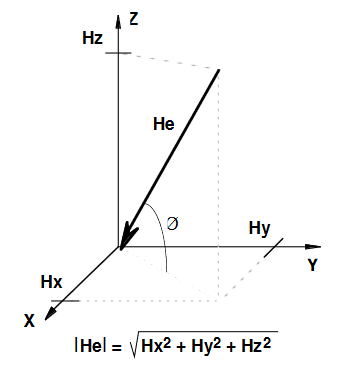
\includegraphics[width=\textwidth]{Figures/fieldaxis.png}
		\caption*{(b) Earth's Field Line ($H_e$) in 3 axes. Source: \cite{magnetometer}}
	\end{minipage}
	\caption{Figure (a) shows Earth's magnetic Field which the sensor is reading on each of the 3 axes - representation about the three axes in (b) of a magnetic field line.}
	\label{figure:earthref}
\end{figure}

The magnetometer reads its orientation relative to the magnetic pole on all three axes. The heading of the robot in degrees can found from $H_x$ and $H_y$ information. Sensor reading are done on a flat surface away from ferrous deposits as these interfere with the sensor. In order to check whether the magnetometer is affected by interference or fabrication defects, readings of the sensor are done on a flat surface while rotating the sensor. The values read should draw a perfect circle as in Figure \ref{figure:cal_uncal_mag} (a). These readings are the maximum and minimum values of the magnetic field line strength on each of the axes. A magnetometer affected by interference or fabrication defects draws a ellipsoid as in Figure \ref{figure:cal_uncal_mag} (b).

\begin{figure}[H]
	\begin{minipage}{0.48\linewidth}
		\centering
		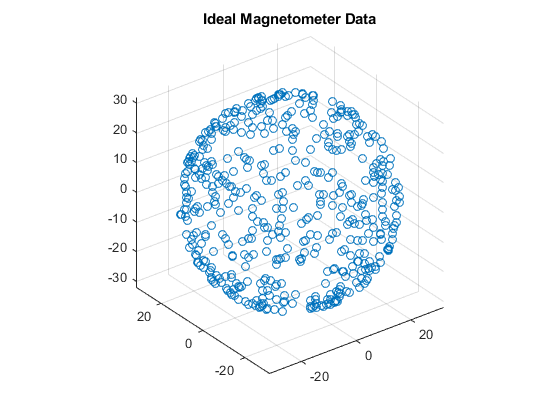
\includegraphics[width=\textwidth]{Figures/perfectcircle.png}
		\caption*{(a) Perfect circle drawn by readings of a calibrated magnetometer.}
	\end{minipage}\hfill
	\begin{minipage}{0.48\linewidth}
		\centering
		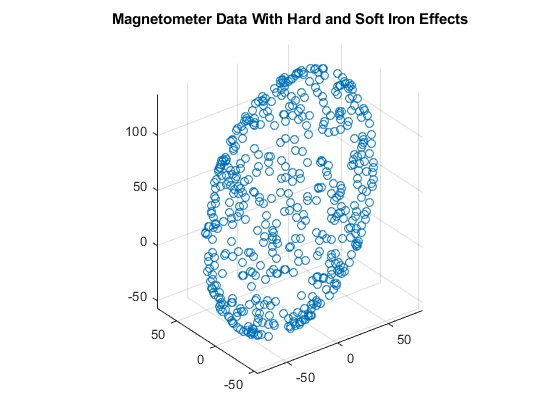
\includegraphics[width=\textwidth]{Figures/ellipsoid.png}
		\caption*{(b) Ellipsoid drawn by readings of an uncalibrated magnetometer.}
	\end{minipage}
	\caption{Figures showing the differences between an uncalibrated (out-of-the-box) magnetometer and a calibrated one. The difference stands in the form drawn by the readings of the magnetometer. Source: \cite{magnetometermatlab}}
	\label{figure:cal_uncal_mag}
\end{figure}

Magnetometer calibration is needed in order to eliminate the effects of the interference. There are two types of interference: hard and soft iron. Hard iron effects refer to the noise sources from the circuit itself or rather fabrication defects. Hard iron effects shift the origin of the circle (2D) or sphere (3D). Soft iron effects come from objects surrounding the magnetometer that distort the magnetic field. These effects stretch and tilt the circle/sphere by making it look like an ellipsoid.\\

Hard iron effects are compensated for by finding the minimum and maximum values for each axis and calculating their average. This average is decreased from each magnetometer axis reading. \\

Soft iron effects are more difficult to eliminate and this involves calculating correction coefficients that multiplied with the magnetometer's readings transforms the ellipsoid in a circle/sphere. The correction coefficient is a scale of the average distance from the centre (radius) divided by the average value of respective axes \cite{magnetometercal}.\\

The calibration algorithm is implemented in the Teensy as shown in snippet \ref{code:magcal}.

\begin{lstlisting}[language=C++, caption={Hard and Soft Iron Effects - Magnetometer Calibration.}, label={code:magcal}]

#include "HMC5883L.h"
HMC5883L mag;

int16_t mx, my, mz;
float mx_cal, my_cal, mz_cal;

const int MAGXMAX = -110;
const int MAGXMIN = -582;
const int MAGYMAX = 395;
const int MAGYMIN = -92;

mag.getHeading(&mx, &my, &mz);

// hard and soft iron calibration for x,y axes
mx_cal=(float)mx-(float)(MAGXMAX+MAGXMIN)/2;
mx_cal=2*mx_cal/((float)(MAGXMAX-MAGXMIN));

my_cal=(float)my-(float)(MAGYMAX+MAGYMIN)/2;
my_cal=2*my_cal/((float)(MAGYMAX-MAGYMIN));


\end{lstlisting}

Once the calibration for each magnetometer axis is done, the heading of the robot is calculated using the $atan2$ function on the $x$ and $y$ axis. As mentioned before, the declination angle of the robot's location can be added to the heading measurement as shown in Listing \ref{code:magnetometer}. The final heading measurement should point to True North. The accuracy of the measurement is compared to the heading calculated with the kinematic equations and the results are shown in the Sanity Check Section below.

%its orientation is given by the rotation around z-axis\\


\begin{lstlisting}[language=C++, caption={Adding declination angle to the heading measurement.}, label={code:magnetometer}]

// Calculate heading when the magnetometer is level, then correct for signs of axis.
  float heading = atan2(mx_cal, my_cal);

// http://www.magnetic-declination.com/
// Magnetic declination at AAU is: 3gr 22' W, which is 3.366667 Degrees, or 0.058759423968 radians.
  float declinationAngle = 0.0587;
  heading += declinationAngle;

// Correct for when signs are reversed.
  if(heading < 0)
    heading += 2*PI;

// Check for wrap due to addition of declination.
  if(heading > 2*PI)
    heading -= 2*PI;

// Convert radians to degrees for readability.
   float headingDegrees= heading * 180/PI;

\end{lstlisting}

\subsection{Sanity Check}

In this section, the comparison between heading accuracy of the robot is verified by testing the robot on a 2 meter distance from a starting to a goal position. The scope is to observe discrepancies between the two sensors in measuring the heading, not controlling to obtain a certain heading. The sanity test has been performed live by communication through serial between Teensy and Matlab to plot the measurements. The heading of the robot should be 0 or 360 degrees. The results are shown in Figure \ref{figure:sanitycheck_magnetometer}.

\begin{figure}[H]
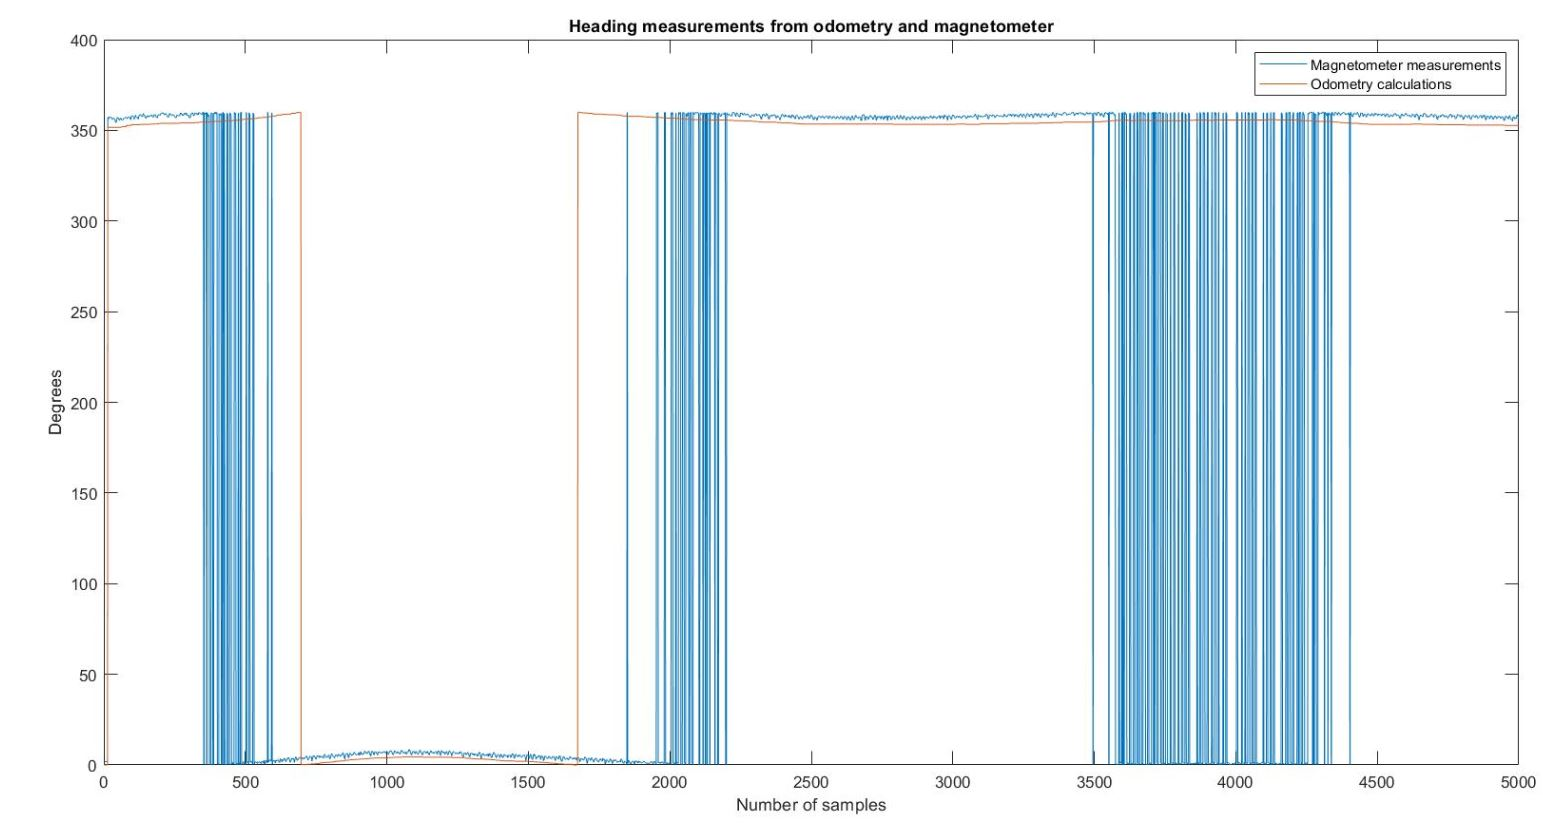
\includegraphics[scale=0.45]{Figures/sanity_check_mag.jpg}
\centering
\caption{Robot heading estimation through encoders versus magnetometer. Heading of robot should be 0 or 360 degrees.}
\label{figure:sanitycheck_mag}
\end{figure}

The results of the sanity test show that the two estimators of the robot's heading are quite good, and a fusion between these two should prevent errors due to magnetic interference or wheel slip from encoder readings.

\section{Chapter Summary}


